\chapter{Design}
\label{chap:design}

Following the analysis developed in the previous chapter (Chapter \ref{chap:analysis}), and after 
a series of design decisions, the final architecture of this master's thesis is shown 
in Figure \ref{fig:project_arch}. This chapter aims to explain the design decisions made, their 
justification, and how they have affected the different modules of the project. All 
these design decisions documented here will lay the foundation for the 
implementation described in Chapter~\ref{chap:implementation}.

\begin{figure}[H]
    \centering
    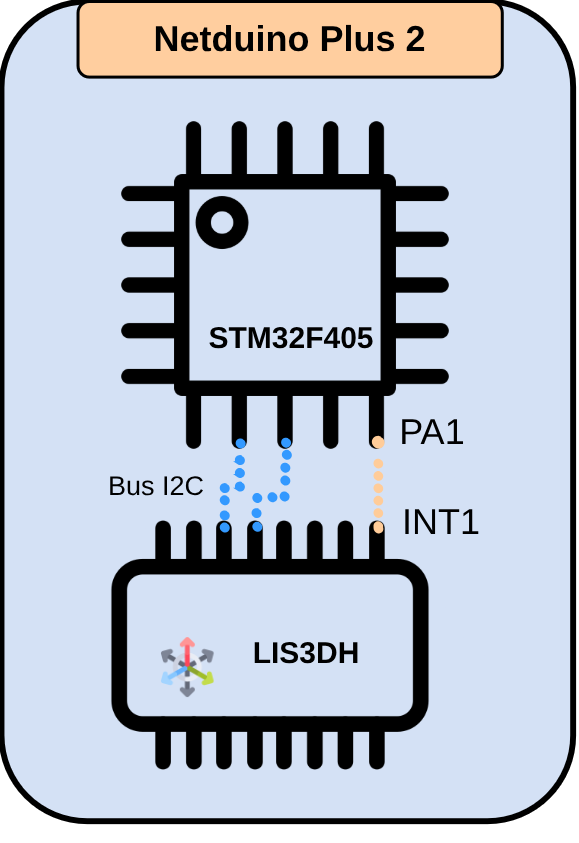
\includegraphics[width=0.45\textwidth]{Resources/Imagenes/my_arch.png}
    \caption{General architecture of the project}
    \label{fig:project_arch}
\end{figure}

%==== Design Decisions ====%
\section{Design Considerations}
\label{chap:design_decisions}

\textbullet\ \textbf{ I$^2$C Master-Only Mode:}

One of the initial design decisions was to focus the development of the 
\\STM32F405's  I$^2$C interface exclusively on master mode. This is because, in the 
educational context in which it will be used, there is no need to use a microcontroller 
as an  I$^2$C slave. Furthermore, the LIS3DH sensor does not have a master mode, so 
this decision defines the operational context in which the STM32F405 communicates 
with the LIS3DH accelerometer. This decision simplifies the scope of the emulation 
while maintaining full functional reliability for the intended use case.

\textbullet\ \textbf{Timing Register Abstraction:}

QEMU implements the  I$^2$C protocol through functions that abstract the different 
events of the  I$^2$C protocol (Code~\ref{code:qemu_i2c_fun}), without requiring cycle-level clock generation. This 
abstraction significantly reduces implementation complexity and preserves functional correctness for firmware testing. 
To emulate the STM32F405 I$^2$C protocol, this means that it is not necessary 
to implement the timing logic controlled by the I2C\_CCR and I2C\_TRISE registers.

\lstinputlisting[
  language=C,
  caption={\texttt{qemu i2c functions}},
  label={code:qemu_i2c_fun}
]{Resources/Code/i2c_functions.c}


\textbullet\ \textbf{Netduino Plus 2 as a Development Board for the STM32F405 Microcontroller:}

Unlike other emulators, QEMU fully emulates a hardware platform; it doesn't 
offer the option to emulate only MCU models independently. This limitation 
created the need to find or implement a development board model in QEMU that 
used the STM32F405 microcontroller. Fortunately, QEMU has a pre-implemented 
minimalist model of the Netduino Plus 2 electronic development board, based on 
the STM32F405RG microcontroller, which has saved users from having to develop 
a new board to implement the microcontroller.

\textbullet\ \textbf{DRDY-Only Interrupt Implementation:}

As explained during the analysis of LIS3DH in section~\ref{chap:analysis_lis3dh}, this accelerometer 
has several interrupts. Of all the interrupts it offers, only the data-ready (DRDY) 
interrupt logic could be implemented. While the goal was to implement the logic 
for all interrupts, the development began with the DRDY interrupt logic due to its 
simplicity and because it represents the most common interrupt mode in embedded 
applications. Unfortunately, due to time constraints, the logic for the remaining 
interrupts could not be implemented. These omissions do not affect the basic 
functionality required for typical STM32 firmware development scenarios, where DRDY 
polling or simple data ready interrupts are sufficient.

\textbullet\ \textbf{QOM as interface:}

Conceived as a temporary solution until its full implementation in MICROLAB, 
the LIS3DH accelerometer model has been designed to allow runtime access to 
acceleration values for each axis. This has been achieved by defining QOM properties 
in the model. As explained during the QEMU analysis, the QOM API allows the 
creation of dynamic properties that can be modified at runtime. Thanks to these 
properties, the developer can inject known acceleration values using commands, such 
as those described in the Figure~\ref{fig:qom_exampe}, to test the accelerometer's functionality with known 
values.

\begin{figure}[H]
    \centering
    \begin{verbatim}
        (qemu) qom-set /machine/soc/i2c[0]/i2c1/child[0] accel-x 500 
        (qemu) qom-set /machine/soc/i2c[0]/i2c1/child[0] accel-y -300 
        (qemu) qom-set /machine/soc/i2c[0]/i2c1/child[0] accel-z 980
        
        (qemu) qom-get /machine/soc/i2c[0]/i2c1/child[0] accel-x 
        500
        (qemu) qom-get /machine/soc/i2c[0]/i2c1/child[0] accel-y 
        -300
        (qemu) qom-get /machine/soc/i2c[0]/i2c1/child[0] accel-z
        980  
    \end{verbatim}
    \caption{access to qom properties}
    \label{fig:qom_exampe}
\end{figure}



\newpage
%==== I2C Controler ====%
\section{\texorpdfstring{I$^2$C Controller Design}{I2C Controller Design}}
\label{chap:design_i2c_controler}


As explained during the analysis, the I$^2$C controller model of the STM32F405 
microcontroller must be able to recognize the specific sequences of register read and 
write operations (Figures~\ref{fig:i2c_master_transmission} \& Figure~\ref{fig:i2c_master_recv}) that the firmware executes on the real 
hardware to generate the I$^2$C protocol events. This condition must be met for the 
emulated hardware to be able to execute the same I$^2$C events in QEMU.

The analysis shows that the generation of I$^2$C events in the controller model 
depends not only on the current state of the registers but also on the previous I$^2$C 
events. This implies that, in addition to implementing the individual logic for each 
register, a finite state machine (FSM) must be implemented, triggered by the register 
reads and writes.

After an extensive reading of the I$^2$C protocol in the STM32F405 
microcontroller reference manual, and following the sequences of Figures~\ref{fig:i2c_master_transmission} and Figure~\ref{fig:i2c_master_recv} 
which are also shown in the same manual, the state machine of Figure \ref{fig:i2c_fsm} 
was reached. In the Table \ref{tab:i2c_fsm_state} are explained every state.


\begin{figure}[H]
    \centering
    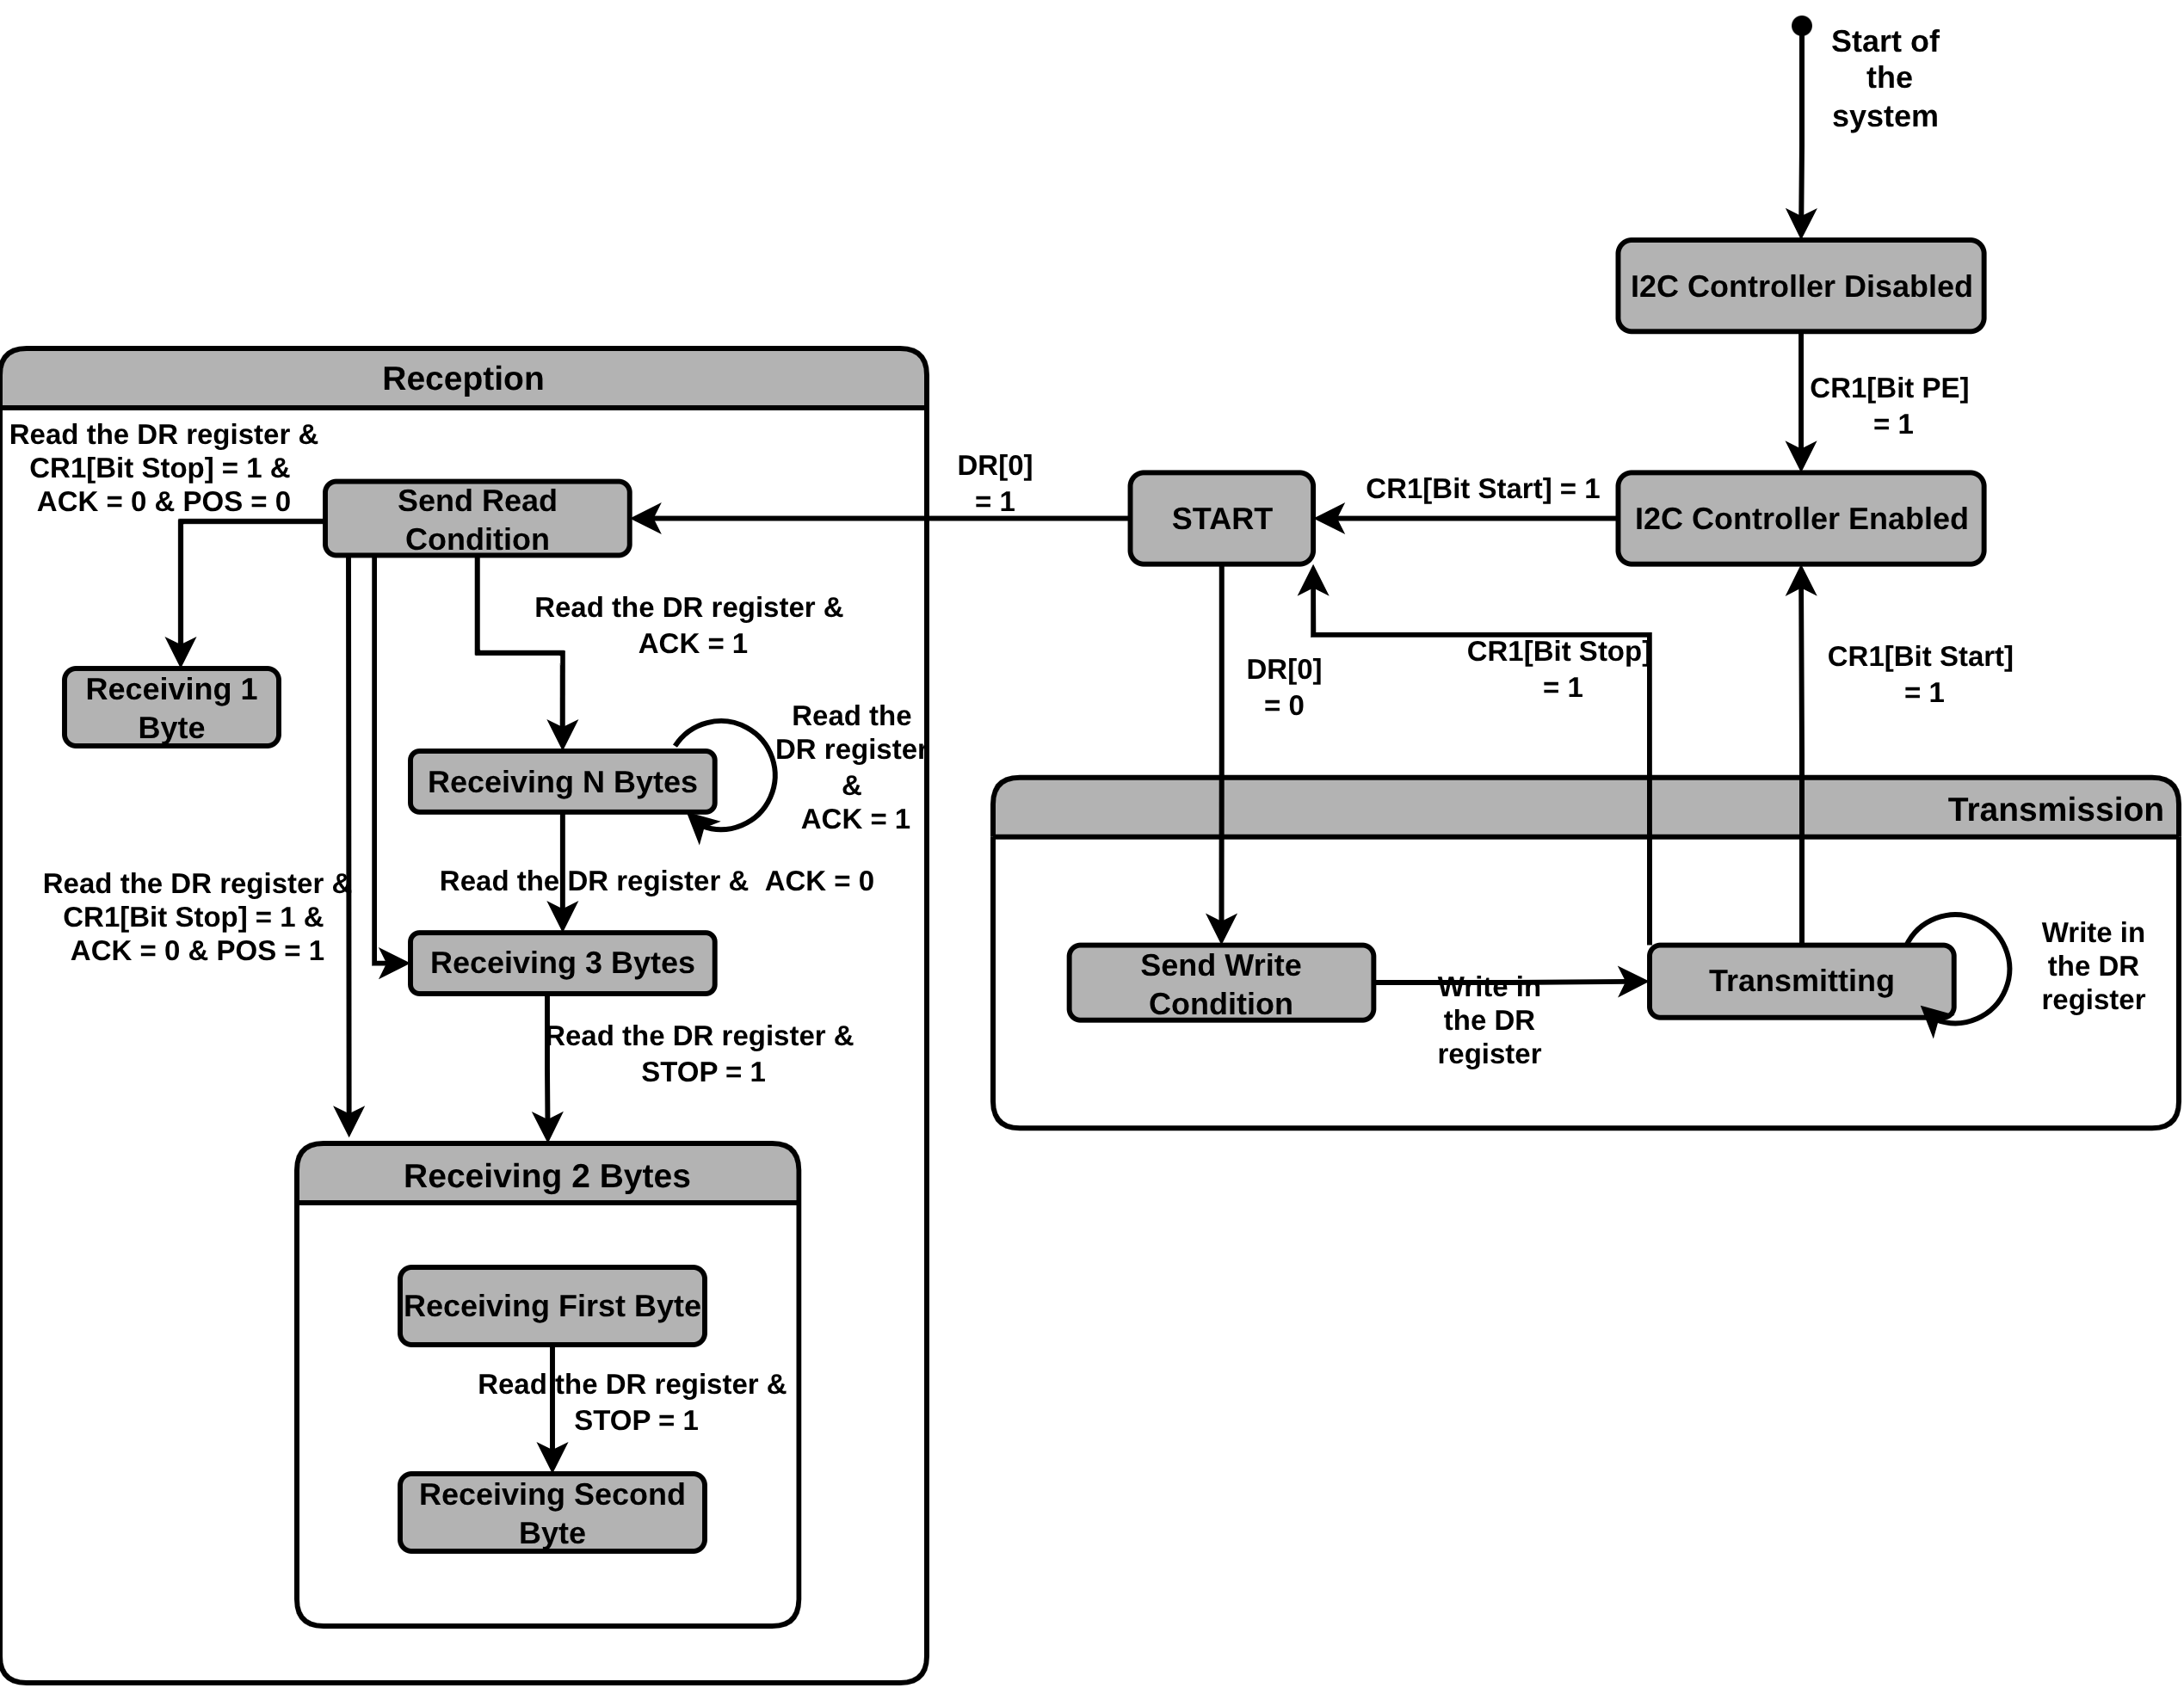
\includegraphics[width=1\textwidth]{Resources/Imagenes/fsm_2.png}
    \caption{stm32f405 i2c controller fsm}
    \label{fig:i2c_fsm}
\end{figure}

\begin{table}[H]
    \small

    \begin{tabularx}{\textwidth}{|c|X|c|X|}
        \hline
        \textbf{Current State}  & \textbf{Transition }  & \textbf{Next State}   & \textbf{Output Action}    \\
                                & \textbf{Condition}    &                       &                           \\
        \hline
        \texttt{DISABLED} & \texttt{CR1[PE] = 1} (Peripheral Enable) & \texttt{IDLE} & Initialize FSM \\
        \hline
        \texttt{IDLE} & \texttt{CR1[START] = 1} & \texttt{START} & Set MSL/BUSY, set SB flag \\
        \hline
        \texttt{START} & \texttt{DR write} (R/W=0) & \texttt{S\_WRITE} & \texttt{i2c\_start\_transfer()}, set ADDR/TXE/BTF \\
        \hline
        \texttt{S\_WRITE} & \texttt{DR write} & \texttt{TRANSMITTING} & \texttt{i2c\_send()}, set TXE/BTF \\
        \hline
        \texttt{TRANSMITTING} & \texttt{DR write} & \texttt{TRANSMITTING} & \texttt{i2c\_send()}, set TXE/BTF \\
        \hline
        \texttt{TRANSMITTING} & \texttt{CR1[START] = 1} & \texttt{START} & Repeated START condition \\
        \hline
        \texttt{TRANSMITTING} & \texttt{CR1[STOP] = 1} & \texttt{IDLE} & \texttt{i2c\_end\_transfer()}, clear flags \\
        \hline
        \texttt{START} & \texttt{DR write} (R/W=1) & \texttt{S\_READ} & \texttt{i2c\_start\_transfer()}, set ADDR/RXNE/BTF \\
        \hline
        \texttt{S\_READ} & \texttt{DR read} \& \texttt{CR1[STOP]=1} \& \texttt{ACK=0} \& \texttt{POS=0} & \texttt{RECV\_1BYTE} & \texttt{i2c\_recv()}, set RXNE/BTF \\
        \hline
        \texttt{S\_READ} & \texttt{DR read} \& \texttt{CR1[STOP]=1} \& \texttt{ACK=0} \& \texttt{POS=1} & \texttt{RECV\_2BYTES\_FIRST} & \texttt{i2c\_recv()}, set RXNE/BTF \\
        \hline
        \texttt{S\_READ} & \texttt{DR read} \& \texttt{ACK=0} \& \texttt{POS=0} & \texttt{RECV\_3BYTES} & \texttt{i2c\_recv()}, set RXNE/BTF \\
        \hline
        \texttt{S\_READ} & \texttt{DR read} \& \texttt{ACK=1} & \texttt{RECV\_NBYTES} & \texttt{i2c\_recv()}, set RXNE/BTF \\
        \hline
        \texttt{RECV\_2BYTES\_FIRST} & \texttt{DR read} \& \texttt{STOP=1} & \texttt{RECV\_2BYTES\_SECOND} & \texttt{i2c\_recv()} (last byte), generate NACK \\
        \hline
        \texttt{RECV\_3BYTES} & \texttt{DR read} \& \texttt{STOP=1} & \texttt{RECV\_2BYTES\_FIRST} & Transition to 2-byte receive mode \\
        \hline
        \texttt{RECV\_NBYTES} & \texttt{DR read} \& \texttt{ACK=1} & \texttt{RECV\_NBYTES} & \texttt{i2c\_recv()}, continue NACK sequence \\
        \hline
        \texttt{RECV\_NBYTES} & \texttt{DR read} \& \texttt{ACK=0} & \texttt{RECV\_3BYTES} & Prepare for 3-byte special case \\
        \hline
        \texttt{RECV\_NBYTES} & \texttt{DR read} \& \texttt{STOP=1} \& \texttt{ACK=0} & \texttt{RECV\_2BYTES\_FIRST} & Final byte handling \\
        \hline
        \texttt{RECV\_1BYTE} & \texttt{STOP=1} & \texttt{IDLE} & \texttt{i2c\_end\_transfer()} \\
        \hline
        \texttt{RECV\_2BYTES\_SECOND} & \texttt{STOP=1} & \texttt{IDLE} & \texttt{i2c\_end\_transfer()} \\
        \hline
    \end{tabularx}



    %\begin{tabular}{|l|p{10cm}|}
    %    \hline
    %    \textbf{State} & \textbf{Description} \\
    %    \hline
    %    DISABLED                & Peripheral disabled (PE bit = 0 in CR1)                       \\
    %    IDLE                    & Peripheral enabled, bus idle, ready to generate START         \\
    %    START                   & START condition generated, waiting for address transmission   \\
    %    SENT\_WRITE             & Address transmitted in write mode, waiting for data or register 
    %                                address \\
    %    SENT\_READ              & Address transmitted in read mode, configuring receive mode    \\
    %    TRANSMITTING            & Actively transmitting data bytes to slave device              \\
    %    RECV\_1BYTE             & Single-byte read mode configured (NACK pre-loaded)            \\
    %    RECV\_2BYTES\_FIRST     & Two-byte read, first byte reception                           \\
    %    RECV\_2BYTES\_SECOND    & Two-byte read, second byte reception                          \\
    %    RECV\_3BYTES            & Three-byte read mode (special NACK timing)                    \\
    %    RECV\_NBYTES            & Multi-byte read mode (N $>$ 3, ACK enabled)                   \\
    %    \hline
    %\end{tabular}

    \caption{STM32F4 I2C Master Mode Finite State Machine Transitions}
    \label{tab:i2c_fsm_state}
\end{table}

\newpage
%==== I2C Controler ====%
\section{LIS3DH Design}
\label{chap:design_lis3dh}

The LIS3DH accelerometer model to be emulated in QEMU has been designed as an I$^2$C slave device, faithfully reproducing the register map and, to a large extent, the configuration logic for all operating parameters (data rate, sensitivity, etc.) defined in the STMicroelectronics datasheet, which were already analyzed in subsection~\ref{chap:analysis_lis3dh} of the analysis chapter (Chapter~\ref{chap:analysis} of this thesis). All of this aims to ensure that the firmware running on the emulated STM32F405 can configure and interact with the LIS3DH identically to the physical hardware.

The logic of the configuration registers has been a crucial element. Although different options were considered, a mechanism was ultimately designed whereby any modification to the control registers immediately recalculates the operating parameters. The following specific functions have been developed to perform the calculation of the internal parameters:

\lstinputlisting[
    language=C,
    caption={lis3dh parameters functions},
    label={fig:lis3dh_parameters_functions}
]{Resources/Code/lis3dh/lis3dh_parameters_fun.c}

One design decision made was to allow developers to directly inject known acceleration values into each axis using QOM properties. These properties are accel-x, accel-y, and accel-z, and represent the acceleration of each axis in milligravity units. The values these properties receive from the developer cannot be directly assigned to the output registers (OUT\_X\_L/H, OUT\_Y\_L/H, and OUT\_Z\_L/H); they must first undergo a three-stage conversion process:

\begin{itemize}
    \item \textbf{Range Validation   :} Input clamped to current FS limits (e.g., ±2000 mg for ±2g mode).
    \item \textbf{Sensitivity Scaling:} Milligravity value divided by mode/FS-specific sensitivity coefficient.
    \item \textbf{Bit-Justification  :} Resulting 16-bit value left-shifted by mode-specific offset (4 bits for High-Res, 6 for Normal, 8 for Low-Power) to match datasheet register layout.
\end{itemize}


This conversion process ensures that the output registers contain bit-precise representations that match the behavior of the physical sensor, allowing the HAL STM32 controllers to correctly avoid modifying the acceleration data.

